\section{Basic Definitions}
%%%%%%%%%%%%%%%%%%%%%%%%%%%%%%%%%%%%%%%%%%%%%%%%%%%%%%%%%%%%%%%%%%%%%%%%%%%%
%%%%%%%%%%%%%%%%%%%%%%%%%%%%%%%%%%%%%%%%%%%%%%%%%%%%%%%%%%%%%%%%%%%%%%%%%%%%
  \begin{frame}{What's \texttt{GNU/Linux}?}{More info:
    \href{https://en.wikipedia.org/wiki/History_of_Linux}{History of GNU/Linux in Wikipedia}}
%-------------------------------------------------------
  \vspace{-0.3cm}
\only<1-2>{
  \begin{columns}[c]
    \column{.75\textwidth}
    \begin{block}{\texttt{GNU/Linux} is an operating system (OS)}
      {\footnotesize By OS we mean the
        software on a computer that enables applications and the computer
        operator to access the devices on the computer to perform desired
        functions. }
    \end{block}
    \column{.25\textwidth}
  \begin{center}
    
\includegraphics[angle=0,width=0.5\linewidth]{./Figs/Tux.png}

  \end{center}
\end{columns}
}
%%%%%%%%%%%%%%%%%%%%%%%%%%%%%%%%%%%%%%%%%%%%%%%%%%%%%%%%%%%%%%%%%%%%%%%%%%%%%%%%%%
\only<2>{
  \begin{columns}[c]
    \column{.4\textwidth}
    \begin{block}{\texttt{GNU/Linux} is a version of the \texttt{UNIX} OS}
      {\footnotesize The \texttt{UNIX} OS was first developed in the 1960s, and has been under constant development ever since. It is a \emph{stable}, \emph{multi-user}, \emph{multi-tasking} system for servers, desktops and laptops. }
    \end{block}
    \column{.6\textwidth}
  \begin{center}
    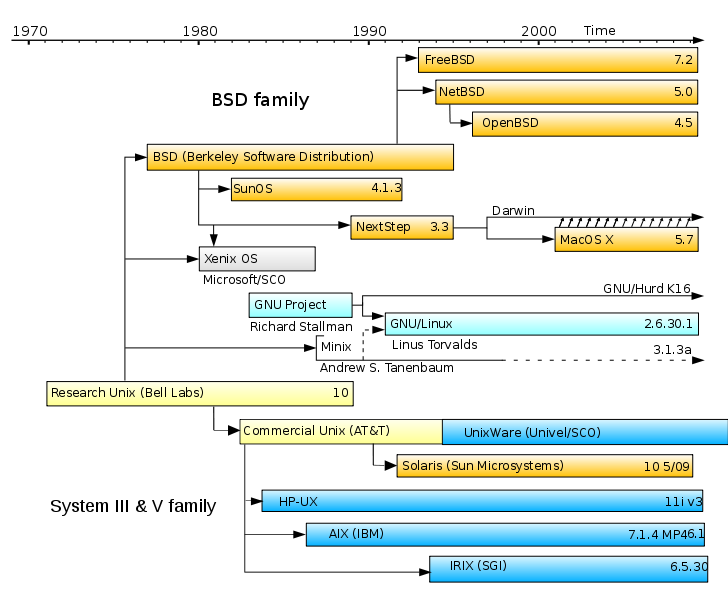
\includegraphics[angle=0,width=0.7\linewidth]{./Figs/Unix_history.png}

  \end{center}
\end{columns}
}
\note{
{\tiny

Notes Module I
}
}
\end{frame}
%%%%%%%%%%%%%%%%%%%%%%%%%%%%%%%%%%%%%%%%%%%%%%%%%%%%%%%%%%%%%%%%%%%%%%%%%%%%%%%%%%%%%%%%%%%
%%%%%%%%%%%%%%%%%%%%%%%%%%%%%%%%%%%%%%%%%%%%%%%%%%%%%%%%%%%%%%%%%%%%%%%%%%%%%%%%%%%%%%%%%%%
\begin{frame}{\texttt{UNIX} components}{Kernel, Shell, and Programs/Apps}
  % -------------------------------------------------------
  \begin{block}{\texttt{UNIX} OS components: \textbf{kernel}, \textbf{shell}, and \textbf{programs/applications}}
    \begin{description}%[Other description]
  \item[Kernel]  {\footnotesize The kernel of UNIX is the hub of the operating system: it allocates time and memory to programs and handles the filestore and communications in response to system calls. }

  \item[Shell]  {\footnotesize The shell is an interface between the user and the kernel. Once a user logs in the shell is started. The shell is a command line interpreter (CLI). It interprets the commands the user types in and arranges for them to be carried out. The commands are themselves programs: when they terminate, the shell gives the user another prompt.}

    {\footnotesize The standard shell in our case is the \alert{\texttt{bash}} shell. The user can customise his shell, and users can use different shells on the same machine.}

  \end{description}

    \end{block}
%%%%%%%%%%%%%%%%%%%%%%%%%%%%%%%%%%%%%%%%%%%%%%%%%%%%%%%%%%%%%%%%%%%%%%%%%%%%%%%%%%
\note{
{\tiny

Notes Module I
}
}
\end{frame}
%%%%%%%%%%%%%%%%%%%%%%%%%%%%%%%%%%%%%%%%%%%%%%%%%%%%%%%%%%%%%%%%%%%%%%%%%%%%
%%%%%%%%%%%%%%%%%%%%%%%%%%%%%%%%%%%%%%%%%%%%%%%%%%%%%%%%%%%%%%%%%%%%%%%%%%%%
\begin{frame}{\texttt{GNU/Linux} Distributions}
  % -------------------------------------------------------
    \begin{itemize}
  \item {\footnotesize \texttt{GNU/Linux} was born as free software and this fact boosted its development and carried out the definition of different \texttt{GNU/Linux} distributions, aka distros.}

  \item {\footnotesize \texttt{GNU/Linux} package sets are called distributions because the \texttt{GNU/Linux} provider or  vendor is distributing an open source operating system that it did not develop from scratch, although it may have enhanced it with its own modifications.}

  \item {\footnotesize   There is a myriad of \texttt{GNU/Linux} distros, including different software and having different ideologies. We have selected \alert{\texttt{Mint 19.1 Tessa}}, that stems from \texttt{Debian Linux}.}
  \item {\footnotesize  For more info see \href{http://distrowatch.com/}{DistroWatch} or \href{http://futurist.se/gldt/}{Distribution Timeline}.}
  \end{itemize}
%%%%%%%%%%%%%%%%%%%%%%%%%%%%%%%%%%%%%%%%%%%%%%%%%%%%%%%%%%%%%%%%%%%%%%%%%%%%%%%%%%
\note{
{\tiny

Notes Module I
}
}
\end{frame}
%%%%%%%%%%%%%%%%%%%%%%%%%%%%%%%%%%%%%%%%%%%%%%%%%%%%%%%%%%%%%%%%%%%%%%%%%%%%
%%%%%%%%%%%%%%%%%%%%%%%%%%%%%%%%%%%%%%%%%%%%%%%%%%%%%%%%%%%%%%%%%%%%%%%%%%%%
\begin{frame}{Starting a terminal in \texttt{Xfce}}
  % -------------------------------------------------------
    \begin{itemize}
  \item {\small \texttt{Xfce} is the default \alert{Window Manager} in the \texttt{Mint 19.1 Tessa} distribution.  There are different ways to start a terminal in \texttt{Xfce}. }

  \item {\small Use the application menu. You can add the terminal entry from the menu to the screen panel.}
  \item {\small Press \texttt{ Alt+F2}, then type \texttt{xfce4-terminal} or \texttt{xterm} to run the terminal.

}

  \item {\small Defining a terminal shortcut}
      \begin{itemize}
    {\footnotesize
    \item Go to \texttt{Applications Menu -> Settings -> Settings Manager}. Find \texttt{Keyboard} and click it.
    \item Go to \texttt{Applications shortcuts} and click \texttt{Add button}
    \item Enter: \texttt{xfce4-terminal} in the command field.
    \item As soon as the \texttt{Command} dialog opens, hit \texttt{Ctrl + Alt + t} (or other keyboard shortcut of your preference).
  }
    \end{itemize}
  \end{itemize}
%%%%%%%%%%%%%%%%%%%%%%%%%%%%%%%%%%%%%%%%%%%%%%%%%%%%%%%%%%%%%%%%%%%%%%%%%%%%%%%%%%
\note{
{\tiny

Notes Module I
}
}
\end{frame}
%%%%%%%%%%%%%%%%%%%%%%%%%%%%%%%%%%%%%%%%%%%%%%%%%%%%%%%%%%%%%%%%%%%%%%%%%%%%
%%%%%%%%%%%%%%%%%%%%%%%%%%%%%%%%%%%%%%%%%%%%%%%%%%%%%%%%%%%%%%%%%%%%%%%%%%%%
\begin{frame}{Why should we bother to work on CLI?}{Apart from being way more cooler...}
  % -------------------------------------------------------
   { Reasons to work with \texttt{GNU/Linux} using a \alert{CLI} (Command Line Interface) better than a GUI (Graphical User Interface).}
   \begin{itemize}
   \item {\small In spite of the many variants of  \texttt{GNU/Linux} and  \texttt{UNIX} the CLI is \alert{common to all of them}. However,  GUIs work differently, with little standardization.}
     
   \item {\small  Command line can appear complicated and daunting, but in the end it resumes in typing, backspacing, cutting, and pasting.}
     
   \item {\small   In spite of the steeper learning curve, the many existing shortcuts and key combinations make in general CLI more powerful that GUI. In particular \texttt{bash-completion} greatly facilitates the user task (\texttt{TAB} = Magic Key).}

   \item {\small  The use of CLI facilitates the work on remote systems and implies a sensitively smaller burden to the computer and the network.
     }
  \end{itemize}
%%%%%%%%%%%%%%%%%%%%%%%%%%%%%%%%%%%%%%%%%%%%%%%%%%%%%%%%%%%%%%%%%%%%%%%%%%%%%%%%%%
\note{
{\tiny

Notes Module I
}
}
\end{frame}
%%%%%%%%%%%%%%%%%%%%%%%%%%%%%%%%%%%%%%%%%%%%%%%%%%%%%%%%%%%%%%%%%%%%%%%%%%%% 
%%%%%%%%%%%%%%%%%%%%%%%%%%%%%%%%%%%%%%%%%%%%%%%%%%%%%%%%%%%%%%%%%%%%%%%%%%%%
\section{The UNIX Filesystem}
%%%%%%%%%%%%%%%%%%%%%%%%%%%%%%%%%%%%%%%%%%%%%%%%%%%%%%%%%%%%%%%%%%%%%%%%%%%%
%%%%%%%%%%%%%%%%%%%%%%%%%%%%%%%%%%%%%%%%%%%%%%%%%%%%%%%%%%%%%%%%%%%%%%%%%%%%
\begin{frame}{A primer on Files and Processes}
  % -------------------------------------------------------

  {Everything in \texttt{UNIX} OS is either a \textbf{file} or a \textbf{process}.}
  
    \begin{itemize}
  \item {\small  A \textbf{process} is an executing program identified by a unique number called its PID (process identifier). }

  \item {\small  A \textbf{file} is a collection of data. They can be created by users using text editors, running compilers, etc.}
    
  \item {\small File examples:}
    \begin{itemize}
      {\footnotesize
      \item a document or text (e.g.\ reports, essays, memos etc.)
      \item a figure or a picture.
      \item the source code of a program written in some high-level programming language.
      \item binary instructions comprehensible directly to the machine, e.g.\ an executable or binary file.
      \item a directory, with information about its contents (files and subdirectories).
      \item special files: \texttt{dev} and \texttt{proc} directories.
      }
    \end{itemize}
  \end{itemize}
%%%%%%%%%%%%%%%%%%%%%%%%%%%%%%%%%%%%%%%%%%%%%%%%%%%%%%%%%%%%%%%%%%%%%%%%%%%%%%%%%%
\note{
{\tiny

Notes Module I
}
}
\end{frame}
%%%%%%%%%%%%%%%%%%%%%%%%%%%%%%%%%%%%%%%%%%%%%%%%%%%%%%%%%%%%%%%%%%%%%%%%%%%%
%%%%%%%%%%%%%%%%%%%%%%%%%%%%%%%%%%%%%%%%%%%%%%%%%%%%%%%%%%%%%%%%%%%%%%%%%%%%
  \begin{frame}{Knowing your filesystem}
%-------------------------------------------------------

    \begin{block}{The root directory}
      The \emph{GNU/Linux} filesystem is hierarchical, the top of the tree
      is the \emph{root} (\alert{/}) directory.
          \end{block}

  % \vspace{-0.3cm}


  \vspace{-0.2cm}
  \begin{columns}[t]
    \column{.5\textwidth}
    \begin{center}
      \vspace{-0.5cm}
      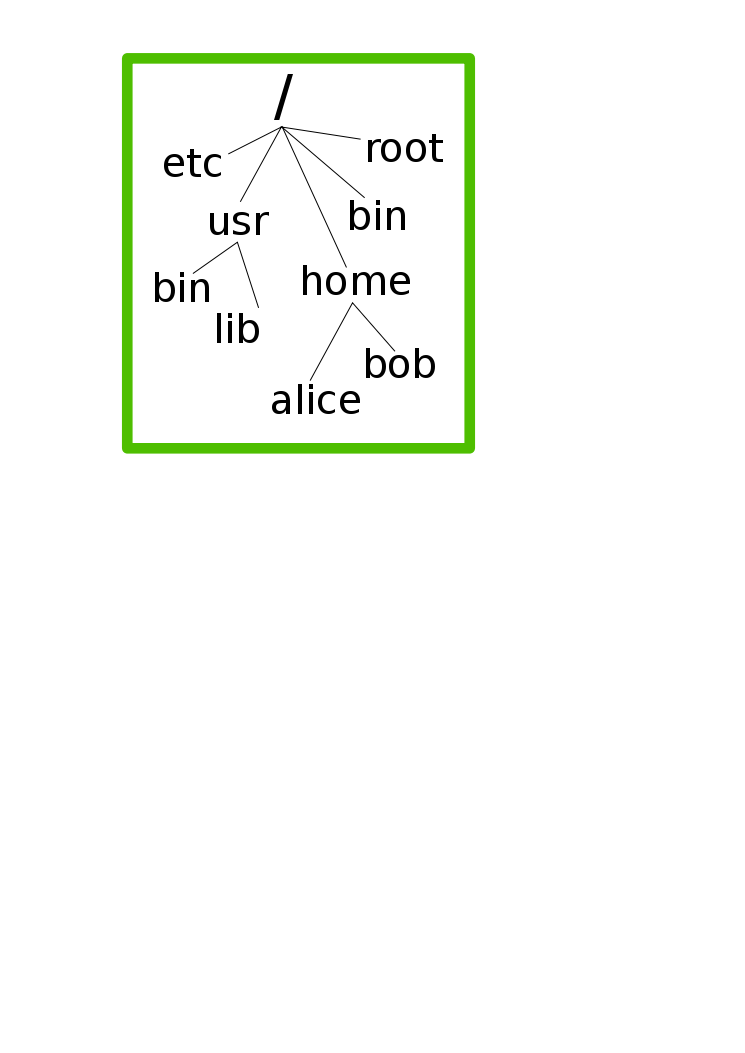
\includegraphics[angle=0,width=\linewidth]{./Figs/drawing.png}
    \end{center}
    \column{.5\textwidth}
    \begin{block}{Basic concepts and commands}
      \begin{itemize}
      \item Concept of path
      \item \texttt{ls} command 
      \item \texttt{cd} command 
      \item \texttt{pwd} command 
      \end{itemize}
    \end{block}
  \end{columns}

      
 \vspace{-5cm}
  \begin{block}
    {\footnotesize The full or absolute path of a file or folder
      locates them starting in the root directory and finishing
      with the file or folder name, e.g.\ \texttt{/home/bob/readme.txt}.}  
  \end{block}

\note{
{\tiny

Notes Module I
}
}
\end{frame}
%%%%%%%%%%%%%%%%%%%%%%%%%%%%%%%%%%%%%%%%%%%%%%%%%%%%%%%%%%%%%%%%%%%%%%%%%%%%
%%%%%%%%%%%%%%%%%%%%%%%%%%%%%%%%%%%%%%%%%%%%%%%%%%%%%%%%%%%%%%%%%%%%%%%%%%%%
\begin{frame}[fragile]{The \texttt{ls} command}
  % -------------------------------------------------------
  
  \begin{block}{ \alert{\texttt{ls}}: list directory contents}
    
    \begin{columns}
      \column{.45\textwidth}
      {\footnotesize By default a console sessions start in the user's home directory, e.g.\ user's \texttt{alice} home directory is \texttt{/home/alice}. The \texttt{ls} command can be used to display the home directory contents.}
    \column{.55\textwidth}
    {\scriptsize
      \begin{lstlisting}
alice@platea:~$ ls
10002.jpg Documents Downloads  
ChemPhys_1_84.pdf nohup.out README
alice@platea:~$
\end{lstlisting}
}
\end{columns}


\vspace{0.5cm}
\begin{columns}
      \column{.45\textwidth}
      {\footnotesize By default \texttt{ls} displays all files besides those that have names starting with a dot ('.'). These are called \alert{hidden files} and usually are system and application configuration files. The option \texttt{-a} makes \texttt{ls} display all files and directories.}
    \column{.55\textwidth}
    {\scriptsize
      \begin{lstlisting}
alice@platea:~$ ls -a
. .. .bash_history .bashrc 
.cache 10002.jpg Documents  Downloads  
ChemPhys_1_84.pdf nohup.out  README
alice@platea:~$
\end{lstlisting}
}
\end{columns}

    \end{block}


\note{
{\tiny

Notes Module I
}
}
\end{frame}
%%%%%%%%%%%%%%%%%%%%%%%%%%%%%%%%%%%%%%%%%%%%%%%%%%%%%%%%%%%%%%%%%%%%%%%%%%%%
%%%%%%%%%%%%%%%%%%%%%%%%%%%%%%%%%%%%%%%%%%%%%%%%%%%%%%%%%%%%%%%%%%%%%%%%%%%%
\begin{frame}[fragile]{The \texttt{cd} command}
  % -------------------------------------------------------
  
  \begin{block}{ \alert{\texttt{cd}}: change to a new working directory}
    
      {\footnotesize  By default you start a session in your home directory (\texttt{/home/username}) and you can make other directory your current directory (working directory) using the \texttt{cd} command.}

    {\scriptsize
      \begin{lstlisting}
alice@platea:~$ ls
10002.jpg  Documents  Downloads ChemPhys_1_84.pdf nohup.out  README
alice@platea:~$ cd /home
alice@platea:/home$ ls
admin alice bob lena pepe
alice@platea:/home$ cd /
alice@platea:/$ ls
bin  cdrom etc  initrd.img media opt  root  sys  usr     vmlinuz
boot dev   home lib lost+found   mnt   proc sbin srv     tmp var
alice@platea:/$
\end{lstlisting}
}

\begin{columns}
      \column{.55\textwidth}
      {\footnotesize There are three important shortcuts that save lots of typing (cool!): '\texttt{.}', current directory; '\texttt{..}', parent directory; and '\textasciitilde', user's home directory.}
    \column{.45\textwidth}
    {\scriptsize
      \begin{lstlisting}
alice@platea:/$ cd ~
alice@platea:~$ cd ..
alice@platea:/home$ cd ./alice
alice@platea:~$ 
\end{lstlisting}
}
\end{columns}

\end{block}


\note{
{\tiny

Notes Module I
}
}
\end{frame}
%%%%%%%%%%%%%%%%%%%%%%%%%%%%%%%%%%%%%%%%%%%%%%%%%%%%%%%%%%%%%%%%%%%%%%%%%%%%
%%%%%%%%%%%%%%%%%%%%%%%%%%%%%%%%%%%%%%%%%%%%%%%%%%%%%%%%%%%%%%%%%%%%%%%%%%%%
\begin{frame}[fragile]{The \texttt{pwd} command}
  % -------------------------------------------------------
  
  \begin{block}{ \alert{\texttt{pwd}}: print working directory absolute path}
    
      {\footnotesize  This command helps the user to locate its current directory. A correct \texttt{bash} prompt definition makes it rarely needed.}

    {\scriptsize
      \begin{lstlisting}
alice@platea:~$ cd /usr/lib
alice@platea:/usr/lib$ pwd
/usr/lib
alice@platea:/usr/lib$ cd
alice@platea:~$ pwd
/home/alice
alice@platea:~$ cd ../../usr/local
alice@platea:/usr/local$ 
      \end{lstlisting}
}

    {\footnotesize
Note that the command \texttt{cd} without arguments is a shortcut for
\\
\texttt{cd /home/username}.
}

\end{block}


\note{
{\tiny

Notes Module I
}
}
\end{frame}
%%%%%%%%%%%%%%%%%%%%%%%%%%%%%%%%%%%%%%%%%%%%%%%%%%%%%%%%%%%%%%%%%%%%%%%%%%%% 
%%%%%%%%%%%%%%%%%%%%%%%%%%%%%%%%%%%%%%%%%%%%%%%%%%%%%%%%%%%%%%%%%%%%%%%%%%%%

\section{Displaying File Contents}
%%%%%%%%%%%%%%%%%%%%%%%%%%%%%%%%%%%%%%%%%%%%%%%%%%%%%%%%%%%%%%%%%%%%%%%%%%%%
%%%%%%%%%%%%%%%%%%%%%%%%%%%%%%%%%%%%%%%%%%%%%%%%%%%%%%%%%%%%%%%%%%%%%%%%%%%%
\begin{frame}[fragile]{Commands that display file contents}
  % -------------------------------------------------------
  
  \begin{block}{ The \alert{\texttt{cat}} and \alert{\texttt{less}} commands}
    
    {\footnotesize
      The contents of \alert{human-readable} (non-binary) files can be displayed using the commands}
%\vspace{0.1cm}

    \begin{center}
  \begin{itemize}
    {\small
\item \alert{\texttt{cat} \emph{filename(s)}}: Concatenate. Automatic scrolling.
\item \alert{\texttt{less} \emph{filename(s)}}: Display file content page by page.
  }
\end{itemize}
\end{center}


{\small The command \texttt{cat} is more adequate for small-size files. In the case of large files, when page scrolling is needed \texttt{less} is the best option. 
\vspace{0.25cm}

The following keys can control the file display with \texttt{less}}
\footnotesize{
\begin{itemize}
\item \texttt{up-arrow}/\texttt{down-arrow}$\leftarrow$ scroll one line at a time. 
\item \texttt{Space}/\texttt{b}$\leftarrow$ scroll one page at a time.
\item \texttt{/}$\leftarrow$ search for a string.
\item \texttt{q}$\leftarrow$ exit \texttt{less}.
\end{itemize}
}

\end{block}


\note{
{\tiny

Notes Module I
}
}
\end{frame}
%%%%%%%%%%%%%%%%%%%%%%%%%%%%%%%%%%%%%%%%%%%%%%%%%%%%%%%%%%%%%%%%%%%%%%%%%%%% 
%%%%%%%%%%%%%%%%%%%%%%%%%%%%%%%%%%%%%%%%%%%%%%%%%%%%%%%%%%%%%%%%%%%%%%%%%%%%

\section{Getting Help}
%%%%%%%%%%%%%%%%%%%%%%%%%%%%%%%%%%%%%%%%%%%%%%%%%%%%%%%%%%%%%%%%%%%%%%%%%%%%
%%%%%%%%%%%%%%%%%%%%%%%%%%%%%%%%%%%%%%%%%%%%%%%%%%%%%%%%%%%%%%%%%%%%%%%%%%%%
\begin{frame}[fragile]{When help is needed...}
  % -------------------------------------------------------
  
  \begin{block}{\alert{\texttt{man}} to the rescue...}
    
    {\small
      The \alert{\texttt{man}} command gives access to a large amount of info about commands and the OS: command syntax and different options.}

    {\footnotesize
    For example, to find out more about the \texttt{ls} command, type
% \vspace{0.1cm}
      \begin{lstlisting}
     alice@platea:~$ man ls
   \end{lstlisting}
   %% $ 
}

    {\footnotesize
Move up and down the man file with the arrow keys, and return to
the command prompt with \alert{\texttt{q}} (Rings a bell with \texttt{less}?). Other alternatives are 
}

{\footnotesize
\vspace{0.15cm}
{\footnotesize
\begin{itemize}
\item \texttt{whatis ls} $\rightarrow$ gives a brief one-line description of the command. \\Same as \texttt{man -f ls}.
\item \texttt{apropos ls} $\rightarrow$ search all man files fro the pattern \texttt{ls}. \\Same as \texttt{man -k ls}.
\item Options \texttt{-h} or \texttt{--help} $\rightarrow$ most commands understand these options.
\end{itemize}
}

The command \alert{\texttt{man intro}} gives a concise and clear introduction to command usage for newbies.}

\end{block}


\note{
{\tiny

Notes Module I
}
}
\end{frame}
%%%%%%%%%%%%%%%%%%%%%%%%%%%%%%%%%%%%%%%%%%%%%%%%%%%%%%%%%%%%%%%%%%%%%%%%%%%% 
%%%%%%%%%%%%%%%%%%%%%%%%%%%%%%%%%%%%%%%%%%%%%%%%%%%%%%%%%%%%%%%%%%%%%%%%%%%%
